% -*- program: xelatex -*-

\newif\ifanswers
%\answerstrue

\documentclass[11pt]{article}

\usepackage{amssymb,amsmath,amsfonts,amsthm,graphicx}
\usepackage[top=0.3in, bottom=0.75in, left=0.5in, right=0.5in]{geometry}
\usepackage{tikz}
\usepackage{array}
\usepackage{enumitem}

\DeclareGraphicsExtensions{.pdf}

\usepackage{fontspec,realscripts}
\defaultfontfeatures{Ligatures=TeX}
\frenchspacing

\usepackage{xcolor}
\usepackage{pagecolor}
\usepackage[document]{ragged2e}

\begin{document}

\noindent
\begin{tabular*}{\textwidth}{@{\extracolsep{\fill}} l r}
\textbf{CS 310: Graph Problems Worksheet}
& \emph{Mudassir Shabbir, May 4, 2026}
\end{tabular*}

\vspace{0.4cm}

\noindent
\begin{tabular*}{\textwidth}{@{\extracolsep{\fill}} l l}
\textbf{Student ID 1 \& 2:}{\em (Do this in pairs)} \hrulefill
&
\end{tabular*}

\vspace{0.3cm}
\hrule
\vspace{0.4cm}

\noindent
\textbf{The Graph $G$.} Work with the following graph $G = (V, E)$ on 9 vertices for all four problems. Dashed edges are part of $G$.

\begin{center}
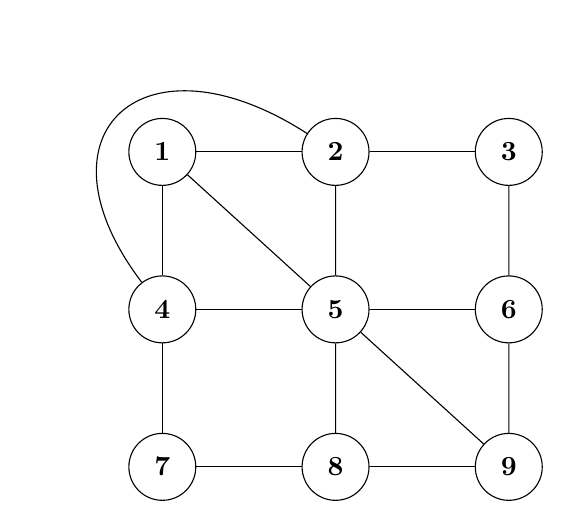
\begin{tikzpicture}[
    every node/.style={circle, draw, minimum size=0.85cm, font=\normalsize\bfseries},
    every edge/.style={draw, thick},
    xscale=2.2, yscale=2.0
]
  % Row 1
  \node (1) at (0,2) {1};
  \node (2) at (1,2) {2};
  \node (3) at (2,2) {3};
  % Row 2
  \node (4) at (0,1) {4};
  \node (5) at (1,1) {5};
  \node (6) at (2,1) {6};
  % Row 3
  \node (7) at (0,0) {7};
  \node (8) at (1,0) {8};
  \node (9) at (2,0) {9};

  % Horizontal edges
  \draw (1)--(2)--(3);
  \draw (4)--(5)--(6);
  \draw (7)--(8)--(9);

  % Vertical edges
  \draw (1)--(4)--(7);
  \draw (2)--(5)--(8);
  \draw (3)--(6)--(9);

  % Diagonal edges
  \draw (1)--(5);
  \draw (5)--(9);
  \draw (2) to[out=145, in=125, looseness=2.2] (4);
\end{tikzpicture}
\end{center}

\vspace{0.3cm}
\hrule
\vspace{0.4cm}

\pagenumbering{gobble}

\begin{enumerate}[leftmargin=0pt, itemindent=1.7em, itemsep=2.2em]

% -----------------------------------------------------------------------
\item \textbf{Minimum Vertex Cover.}

Find a minimum vertex cover of $G$ and argue it is minimum.

\vspace{4cm}

\ifanswers
\textbf{Answer.} $S = \{2,4,5,6,8\}$, $|S|=5$.

\medskip\noindent\textit{Valid cover:} Check each edge has an endpoint in $S$:
horizontal: $1$-$2$ ($2\!\in\!S$), $2$-$3$ ($2\!\in\!S$), $4$-$5$ ($4,5\!\in\!S$), $5$-$6$ ($5,6\!\in\!S$), $7$-$8$ ($8\!\in\!S$), $8$-$9$ ($8\!\in\!S$);
vertical: $1$-$4$ ($4\!\in\!S$), $2$-$5$ ($2,5\!\in\!S$), $3$-$6$ ($6\!\in\!S$), $4$-$7$ ($4\!\in\!S$), $5$-$8$ ($5,8\!\in\!S$), $6$-$9$ ($6\!\in\!S$);
diagonal: $1$-$5$ ($5\!\in\!S$), $5$-$9$ ($5\!\in\!S$), $2$-$4$ ($2,4\!\in\!S$). All edges covered. \checkmark

\medskip\noindent\textit{Minimality:} $I = V\setminus S = \{1,3,7,9\}$ is an independent set of size 4 (verified in Problem 2). Since $|$min VC$| + |$max IS$| = 9$, we get min VC $\le 9-4=5$. Hence $S$ is minimum.
\fi

\newpage

% -----------------------------------------------------------------------
\item \textbf{Maximum Independent Set.}

Find a maximum independent set of $G$.

\vspace{4cm}

\ifanswers
\textbf{Answer.} $I = \{1,3,7,9\}$, $|I|=4$.

\medskip\noindent\textit{Valid:} No edge of $G$ connects two members of $I$: $1$-$3$? No. $1$-$7$? No. $1$-$9$? No. $3$-$7$? No. $3$-$9$? No. $7$-$9$? No. Independent. \checkmark

\medskip\noindent\textit{Maximum:} The complement $V\setminus I = \{2,4,5,6,8\}$ is a vertex cover of size 5 (verified in Problem 1). Any independent set of size 5 would leave only 4 nodes as a vertex cover, but node 5 alone has degree 6, so removing 5 from the cover leaves 6 uncoverable edges — a contradiction. Hence $|I|=4$ is maximum.
\fi

\vspace{4cm}

% -----------------------------------------------------------------------
\item \textbf{Maximum Clique.}

Find a maximum clique of $G$ and show no larger clique exists.

\vspace{4cm}

\ifanswers
\textbf{Answer.} $C = \{1,2,4,5\}$, $|C|=4$.

\medskip\noindent\textit{Valid:} Check all $\binom{4}{2}=6$ pairs: $1$-$2$ (horizontal), $1$-$4$ (vertical), $1$-$5$ (diagonal), $2$-$4$ (dashed), $2$-$5$ (vertical), $4$-$5$ (horizontal). All six edges exist. \checkmark

\medskip\noindent\textit{No $K_5$:} A fifth vertex $x$ would need to be adjacent to all of $1,2,4,5$. But $N(1)=\{2,4,5\}$, so $x\in N(1)\setminus\{2,4,5\}=\emptyset$. Hence $\omega(G)=4$.
\fi

% \newpage

% -----------------------------------------------------------------------
\item \textbf{Maximum Matching.}

Find a maximum matching of $G$.

\vspace{6cm}

\ifanswers
\textbf{Answer.} $M = \{1\text{-}2,\;4\text{-}7,\;5\text{-}6,\;8\text{-}9\}$, $|M|=4$.

\medskip\noindent\textit{Valid:} All four edges exist in $G$. The eight endpoints $\{1,2,4,5,6,7,8,9\}$ are pairwise distinct, so no two edges share a vertex. Vertex 3 is unmatched.

\medskip\noindent\textit{Maximum:} Since $|V|=9$, any matching has $|M|\le\lfloor 9/2\rfloor = 4$. This matching achieves 4, so $\nu(G)=4$.
\fi

\end{enumerate}

\end{document}
